\documentclass[11pt,UTF8]{ctexart}

\usepackage[margin=2cm,a4paper]{geometry}
%\usepackage[left=0.75in,top=0.6in,right=0.75in,bottom=1.0in,a4paper]{geometry}

\setmainfont{Caladea}
%% 也可以選用其它字庫:
% \setCJKmainfont[%
%   ItalicFont=AR PL KaitiM GB,
%   BoldFont=Noto Sans CJK SC,
% ]{Noto Serif CJK SC}
% \setCJKsansfont{Noto Sans CJK SC}
% \renewcommand{\kaishu}{\CJKfontspec{AR PL KaitiM GB}}

% 繁體中文
\setCJKmainfont[Path=fonts/ ]{NotoSansTC-Medium.otf}

\usepackage{minted}
\usepackage[breaklinks]{hyperref}

% Picture
% 導言區的此三行無變化
\usepackage{graphicx}
\usepackage{float} 
\usepackage{subfigure}
% 以下是新增的自定義格式更改
\usepackage[]{caption2} %新增調用的宏包
\renewcommand{\figurename}{Fig.} %重定義編號前綴詞
\renewcommand{\captionlabeldelim}{.~} %重定義分隔符
 %\roman 是羅馬數字編號,\alph是默認的字母編號,\arabic是阿拉伯數字編號,可按需替換下一行的相應位置
\renewcommand{\thesubfigure}{(\roman{subfigure})}%此外,還可設置圖編號顯示格式,加括號或者不加括號
\makeatletter \renewcommand{\@thesubfigure}{\thesubfigure \space}%子圖編號與名稱的間隔設置
\renewcommand{\p@subfigure}{} \makeatother

% Math
\usepackage {mathtools}
\usepackage{amssymb}

% Code
\usepackage{listings}
\usepackage{xcolor}
\lstset{
    % backgroundcolor=\color{red!50!green!50!blue!50},
    % 程式碼塊背景色為淺灰色
    rulesepcolor= \color{gray}, % 程式碼塊邊框顏色
    breaklines=true,  % 程式碼過長則換行
    numbers=left, % 行號在左側顯示
    numberstyle= \small,% 行號字型
    % eywordstyle= \color{red,% 關鍵字顏色
    commentstyle=\color{gray}, % 註釋顏色
    frame=shadowbox % 用方框框住程式碼塊
    }

\usepackage{hyperref}

\title{計算機視覺作業}
\author{干皓丞,2101212850, 信息工程學院}

\begin{document}
\maketitle


\section{作業目標與章節摘要}

根據 W6\_MNIST\_FC.ipynb 改良程式碼好獲得更好的效果。在此可以使用增加卷積層結構,或者嘗試增加 dropout 或者 BN 技術等,訓練出盡可能高的 MNIST 分類效果,原始程式碼在名為 kancheng/kan-cs-report-in-2021 的 Github 專案下,可以在 CV/pytorch-tensorflow-mnist/code 下找到。該報告第一節為 Pytorch MNIST Training 課堂程式碼改良, 第二節為 TensorFlow MNIST Training,第三節為 CNN 方法與重要文獻,而附件則為 Pytorch MNIST Training 中的測試結果。

\begin{figure}[H]
\centering 
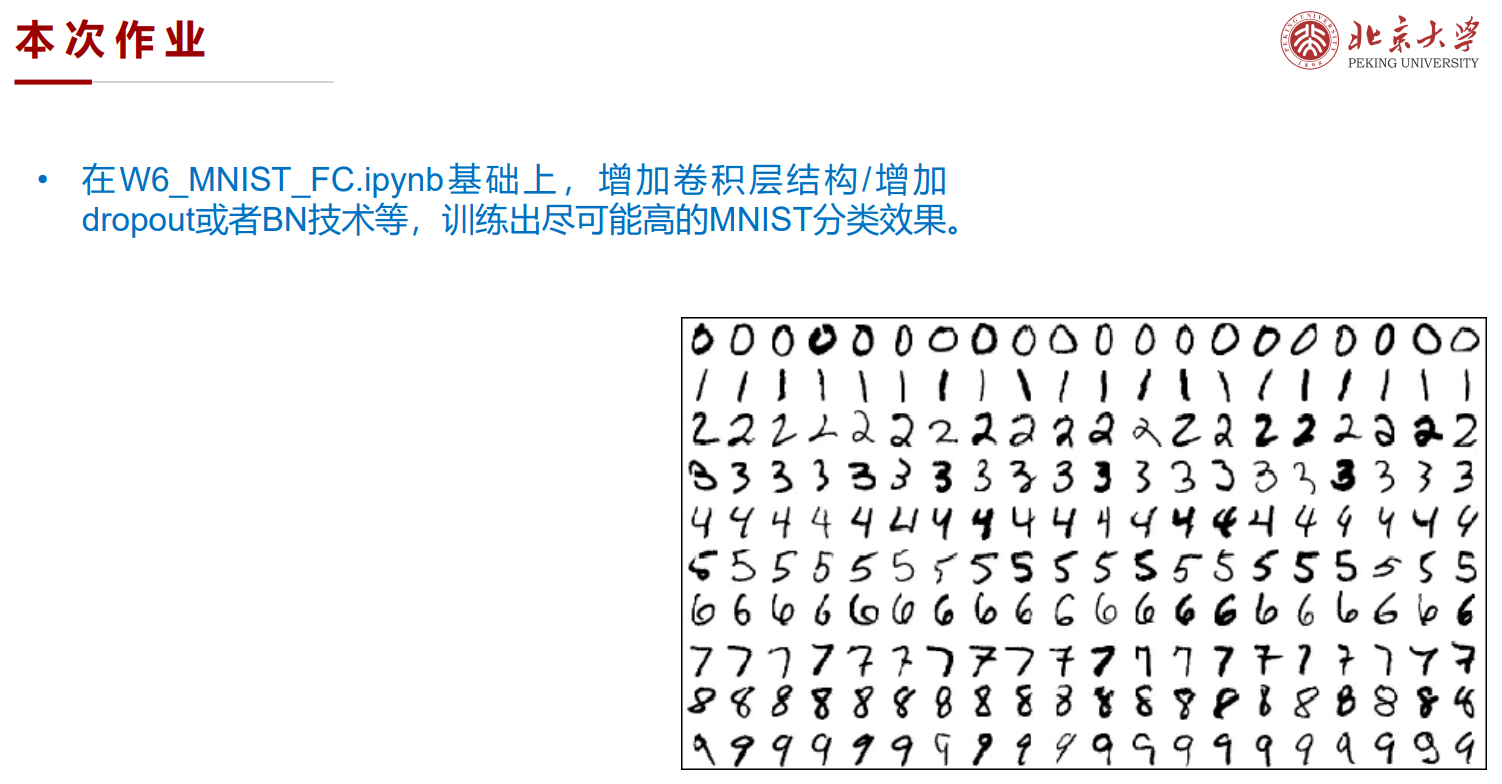
\includegraphics[width=0.9\textwidth]{t1.png} 
\caption{作業目標}
\label{Test}
\end{figure}

\newpage

\section{Pytorch MNIST Training}

Pytorch MNIST Training 原始的範例程式碼中 Test Accuracy 結果為 0.914,而自己 MacBook Pro (Retina, 15-inch, Mid 2014) 實際測試後,在預設值 EPOCH = 2 與 LR = 0.001 所跑出的  Test Accuracy 結果為 0.894 and 0.901。原始程式碼範例如下所示 :

	\begin{lstlisting}[language={python}]
import torch
import torch.nn as nn
import torch.utils.data as Data
import torchvision
import torch.nn.functional as F
import numpy as np
# torch.manual_seed(1)
EPOCH = 2
LR = 0.001
DOWNLOAD_MNIST = True

train_data = torchvision.datasets.MNIST(root='./mnist/', train=True, transform=torchvision.transforms.ToTensor(),
                                        download=DOWNLOAD_MNIST, )
test_data = torchvision.datasets.MNIST(root='./mnist/', train=False)
train_x = torch.unsqueeze(train_data.data, dim=1).type(torch.FloatTensor) / 255.
train_y = train_data.targets
print(train_x.shape)
test_x = torch.unsqueeze(test_data.data, dim=1).type(torch.FloatTensor)[:2000] / 255.  # Tensor on GPU
test_y = test_data.targets[:2000]
test_x.shape
import matplotlib.pyplot as plt
plt.imshow(test_x[1,0,:,:].numpy(), 'gray')
test_y[:10]
class FC(nn.Module):
    def __init__(self):
        super(FC, self).__init__()
        self.fc1 = nn.Linear(784, 256)
        self.fc2 = nn.Linear(256, 10)
        self.fc3 = nn.Linear(10, 10)

    def forward(self, x):
        x = x.view(x.size(0), -1)
        x = self.fc1(x)
        x = F.relu(x)
        x = self.fc2(x)
        x = F.relu(x)
        x = self.fc3(x)

        output = x
        return output


fc = FC()

optimizer = torch.optim.Adam(fc.parameters(), lr=LR)
# loss_func = nn.MSELoss()
loss_func = nn.CrossEntropyLoss()

data_size = 20000
batch_size = 50

for epoch in range(EPOCH):
    random_indx = np.random.permutation(data_size)
    for batch_i in range(data_size // batch_size):
        indx = random_indx[batch_i * batch_size:(batch_i + 1) * batch_size]

        b_x = train_x[indx, :]
        b_y = train_y[indx]
#         print(b_x.shape)
#         print(b_y.shape)

        output = fc(b_x)
        loss = loss_func(output, b_y)

        loss.backward()
        optimizer.step()
        optimizer.zero_grad()

        if batch_i % 50 == 0:
            test_output = fc(test_x)
            pred_y = torch.max(test_output, 1)[1].data.squeeze()
            # pred_y = torch.max(test_output, 1)[1].data.squeeze()
            accuracy = torch.sum(pred_y == test_y).type(torch.FloatTensor) / test_y.size(0)
            print('Epoch: ', epoch, '| train loss: %.4f' % loss.data.cpu().numpy(), '| test accuracy: %.3f' % accuracy)

test_output = fc(test_x[:10])
pred_y = torch.max(test_output, 1)[1].data.squeeze()  # move the computation in GPU

print(pred_y, 'prediction number')
print(test_y[:10], 'real number')

test_output = fc(test_x[:1])
pred_y = torch.max(test_output, 1)[1].data.squeeze()  # move the computation in GPU

print(pred_y, 'prediction number')
print(test_y[:1], 'real number')
test_output
test_x[:1].shape
plt.imshow(test_x[:1].numpy().squeeze(), 'gray')

import torch
torch.eye(10)
0, 1, 2, ..., 9
	\end{lstlisting}


在此針對 FC class 和 batch\_size 進行測試,一開始的 FC 則稱之為 FC3 。FC 為控制訓練的層,而所謂的 Batch Size 為一個重要參數,該參數的意義在於做出在記憶體效率跟記憶體容量之間尋找最佳平衡,若編號為 FC3 且 Batch Size 為 50 則編號表述為 FC3-batch-50。此次實驗共有 FC3、FC4-1、FC4-2、FC7,Batch Size 為 10、30、50。

% 實機測試的 Test Accuracy 為 0.894。而後續測試編號以此類推。

	\begin{lstlisting}[language={python}]
# FC3
class FC(nn.Module):
    def __init__(self):
        super(FC, self).__init__()
        self.fc1 = nn.Linear(784, 256)
        self.fc2 = nn.Linear(256, 10)
        self.fc3 = nn.Linear(10, 10)

    def forward(self, x):
        x = x.view(x.size(0), -1)
        x = self.fc1(x)
        x = F.relu(x)
        x = self.fc2(x)
        x = F.relu(x)
        x = self.fc3(x)
        output = x
        return output
fc = FC()
	\end{lstlisting}

此 FC 則稱之為 FC4-1 。

	\begin{lstlisting}[language={python}]
# FC4-1
class FC(nn.Module):
    def __init__(self):
        super(FC, self).__init__()
        self.fc1 = nn.Linear(784, 256)
        self.fc2 = nn.Linear(256, 128)
        self.fc3 = nn.Linear(128, 10)
        self.fc4 = nn.Linear(10, 10)

    def forward(self, x):
        x = x.view(x.size(0), -1)
        x = self.fc1(x)
        x = F.relu(x)
        x = self.fc2(x)
        x = F.relu(x)
        x = self.fc3(x)
        x = F.relu(x)
        x = self.fc4(x)
        x = F.relu(x)
        output = x
        return output
fc = FC()
	\end{lstlisting}

此 FC 則稱之為 FC4-2 。

	\begin{lstlisting}[language={python}]
# FC4-2
class FC(nn.Module):
    def __init__(self):
        super(FC, self).__init__()
        self.fc1 = nn.Linear(784, 1256)
        self.fc2 = nn.Linear(1256, 128)
        self.fc3 = nn.Linear(128, 10)
        self.fc4 = nn.Linear(10, 10)

    def forward(self, x):
        x = x.view(x.size(0), -1)
        x = self.fc1(x)
        x = F.relu(x)
        x = self.fc2(x)
        x = F.relu(x)
        x = self.fc3(x)
        x = F.relu(x)
        x = self.fc4(x)
        x = F.relu(x)
        output = x
        return output
fc = FC()
	\end{lstlisting}

此 FC 則稱之為 FC7 。

	\begin{lstlisting}[language={python}]
# FC7
class FC(nn.Module):
    def __init__(self):
        super(FC, self).__init__()
        self.fc1 = nn.Linear(784, 256)
        self.fc2 = nn.Linear(256, 128)
        self.fc3 = nn.Linear(128, 64)
        self.fc4 = nn.Linear(64, 32)
        self.fc5 = nn.Linear(32, 16)
        self.fc6 = nn.Linear(16, 10)
        self.fc7 = nn.Linear(10, 10)

    def forward(self, x):
        x = x.view(x.size(0), -1)
        x = self.fc1(x)
        x = F.relu(x)
        x = self.fc2(x)
        x = F.relu(x)
        x = self.fc3(x)
        x = F.relu(x)
        x = self.fc4(x)
        x = F.relu(x)
        x = self.fc5(x)
        x = F.relu(x)
        x = self.fc6(x)
        x = F.relu(x)
        x = self.fc7(x)
        output = x
        return output
fc = FC()
	\end{lstlisting}
	
結果由下表所示,在 FC7 在 Batch Size 為 50 的情況下,效果並不是很理想,跟 FC3的 結果相近,反而是 FC4-1 跟 FC4-2 這兩者有著不錯的表現。前者 FC4-1 在 Batch Size 為 50 時有 0.954,在 Batch Size 為 30 時, FC4-1 第一次實機測試有 0.941,而第二次實機測試則有 0.930,FC4-2 則在 Batch Size 為 30 時做到 0.961。其他詳細結果放在附件 1 與 附件 2 。

\begin{center}
\begin{tabular}{cccccc}
\hline
FC 代號 & Epoch & Train Loss & Test Accuracy & Batch Size & 備註 \\
\hline
FC3 & 1 & 0.2856 & 0.894 & 50 &  \\
FC3 & 1 & 0.3801 & 0.913 & 50 &  \\
FC4-1 & 1 & 0.1782 & 0.954  & 50 & \\
FC7 & 1 & 0.2008 & 0.886 & 50 & \\
FC4-1 & 1 & 0.2815 & 0.941 & 30 & \\
FC4-1 & 1 & 0.0679 & 0.930 & 30 & \\
FC4-2 & 1 & 0.0153 & 0.961 & 30 & \\
FC7 & 1 & 0.0089 & 0.928 & 10 & \\
\hline
\end{tabular}
\end{center}

在此測試只是單純的增加層,而且該測試並無做到相當全面的程度,實際上還可 在投入 dropout 或者 BN 技術等,應該能夠得到更好的效果,。接下來加入卷積並將 EPOCH 設為 10,其範例可以在專案目錄中的 mnist-convolutional.ipynb 找到,其改動程式碼如下 :

	\begin{lstlisting}[language={python}]
import torch
import torch.nn as nn
import torch.utils.data as Data
import torchvision
import torch.nn.functional as F
import numpy as np

# torch.manual_seed(1)

EPOCH = 10
LR = 0.001
DOWNLOAD_MNIST = True

train_data = torchvision.datasets.MNIST(root='./mnist/', train=True, transform=torchvision.transforms.ToTensor(),
                                        download=DOWNLOAD_MNIST, )
test_data = torchvision.datasets.MNIST(root='./mnist/', train=False)


train_x = torch.unsqueeze(train_data.data, dim=1).type(torch.FloatTensor) / 255.
train_y = train_data.targets
print(train_x.shape)

test_x = torch.unsqueeze(test_data.data, dim=1).type(torch.FloatTensor)[:2000] / 255.  # Tensor on GPU
test_y = test_data.targets[:2000]
test_x.shape
import matplotlib.pyplot as plt
plt.imshow(test_x[1,0,:,:].numpy(), 'gray')
# 繪製多個 train_data
figure = plt.figure(figsize=(10, 8))
cols, rows = 5, 5
for i in range(1, cols * rows + 1):
    sample_idx = torch.randint(len(train_data), size=(1,)).item()
    img, label = train_data[sample_idx]
    figure.add_subplot(rows, cols, i)
    plt.title(label)
    plt.axis("off")
    plt.imshow(img.squeeze(), cmap="gray")
plt.show()
test_y[:10]
class FC(nn.Module):
    def __init__(self):
        super(FC, self).__init__()
        self.conv1 = nn.Sequential(         
            nn.Conv2d(
                in_channels=1,              
                out_channels=16,            
                kernel_size=5,              
                stride=1,                   
                padding=2,                  
            ),                              
            nn.ReLU(),                      
            nn.MaxPool2d(kernel_size=2),    
        )
        self.conv2 = nn.Sequential(         
            nn.Conv2d(16, 32, 5, 1, 2),     
            nn.ReLU(),                      
            nn.MaxPool2d(2),                
        )
        self.out = nn.Linear(32 * 7 * 7, 10)

    def forward(self, x):
        x = self.conv1(x)
        x = self.conv2(x)
        # flatten the output of conv2 to (batch_size, 32 * 7 * 7)
        x = x.view(x.size(0), -1)       
        output = self.out(x)
        return output
fc = FC()   
optimizer = torch.optim.Adam(fc.parameters(), lr=LR)
#loss_func = nn.MSELoss()
loss_func = nn.CrossEntropyLoss()

data_size = 50000
batch_size = 50
for epoch in range(EPOCH):
    random_indx = np.random.permutation(data_size)
    for batch_i in range(data_size // batch_size):
        indx = random_indx[batch_i * batch_size:(batch_i + 1) * batch_size]

        b_x = train_x[indx, :]
        b_y = train_y[indx]
#         print(b_x.shape)
#         print(b_y.shape)
        output = fc(b_x)
        loss = loss_func(output, b_y)
        loss.backward()
        optimizer.step()
        optimizer.zero_grad()

        if batch_i % 50 == 0:
            test_output = fc(test_x)
            pred_y = torch.max(test_output, 1)[1].data.squeeze()
            # pred_y = torch.max(test_output, 1)[1].data.squeeze()
            accuracy = torch.sum(pred_y == test_y).type(torch.FloatTensor) / test_y.size(0)
            print('Epoch: ', epoch, '| train loss: %.4f' % loss.data.cpu().numpy(), '| test accuracy: %.3f' % accuracy)

test_output = fc(test_x[:10])
pred_y = torch.max(test_output, 1)[1].data.squeeze()  # move the computation in GPU

print(pred_y, 'prediction number')
print(test_y[:10], 'real number')
test_output = fc(test_x[:1])
pred_y = torch.max(test_output, 1)[1].data.squeeze()  # move the computation in GPU

print(pred_y, 'prediction number')
print(test_y[:1], 'real number')

test_output
test_x[:1].shape
plt.imshow(test_x[:1].numpy().squeeze(), 'gray')
import torch
torch.eye(10)
0, 1, 2, ..., 9
	\end{lstlisting}

結果由下表所示,新的版本加入卷積與改良後,在 Batch Size 為 50,EPOCH 設為 10,LR 設為 0.01,在 EPOCH 跑到 1 時,Test Accuracy 就已經到了 0.976,在 EPOCH 跑到 2 時,Test Accuracy 就已經到了 0.980,過程中 Test Accuracy 曾經到 0.989,EPOCH 跑到 9 結束時,Test Accuracy 最後到達 0.984。在此將實際結果最後一個值列在下表,同時詳細結果放在附件 3。

\begin{center}
\begin{tabular}{ccccc}
\hline
Epoch & Train Loss & Test Accuracy & Batch Size & 備註 \\
\hline
0 & 0.1125 & 0.973 & 50 &  \\
1 & 0.0183 & 0.982 & 50 &  \\
2 & 0.0788 & 0.982 & 50 & \\
3 & 0.0082 & 0.984 & 50 &  \\
4 & 0.0563 & 0.984 & 50 &  \\
5 & 0.0365 & 0.983 & 50 &  \\
6 & 0.0039 & 0.986 & 50 &  \\
7 & 0.0569 & 0.986 & 50 &  \\
8 & 0.0004 & 0.989 & 50 &  \\
9 & 0.0641 & 0.984 & 50 &  \\
\hline
\end{tabular}
\end{center}

% \newpage
\newpage

\section{Tensorflow MNIST Training}

Tensorflow MNIST Training 的 Code 為 Google 在其 Tensorflow 平臺的官方範例嘗試,而環境部屬則與 Pytorch 相似,在此則不詳述。

	\begin{lstlisting}[language={python}]
# Training a neural network on MNIST with Keras
import tensorflow as tf
import tensorflow_datasets as tfds
(ds_train, ds_test), ds_info = tfds.load(
    'mnist',
    split=['train', 'test'],
    shuffle_files=True,
    as_supervised=True,
    with_info=True,
)

show = tfds.show_examples(ds_test, ds_info)

print("Number of original training examples:", len(ds_train))
print("Number of original test examples:", len(ds_test))

def normalize_img(image, label):
  """Normalizes images: `uint8` -> `float32`."""
  return tf.cast(image, tf.float32) / 255., label

ds_train = ds_train.map(
    normalize_img, num_parallel_calls=tf.data.AUTOTUNE)
ds_train = ds_train.cache()
ds_train = ds_train.shuffle(ds_info.splits['train'].num_examples)
ds_train = ds_train.batch(128)
ds_train = ds_train.prefetch(tf.data.AUTOTUNE)
ds_test = ds_test.map(
    normalize_img, num_parallel_calls=tf.data.AUTOTUNE)
ds_test = ds_test.batch(128)
ds_test = ds_test.cache()
ds_test = ds_test.prefetch(tf.data.AUTOTUNE)

model = tf.keras.models.Sequential([
  tf.keras.layers.Flatten(input_shape=(28, 28)),
  tf.keras.layers.Dense(128, activation='relu'),
  tf.keras.layers.Dense(10)
])
model.compile(
    optimizer=tf.keras.optimizers.Adam(0.001),
    loss=tf.keras.losses.SparseCategoricalCrossentropy(from_logits=True),
    metrics=[tf.keras.metrics.SparseCategoricalAccuracy()],
)

model.fit(
    ds_train,
    epochs=6,
    validation_data=ds_test,
)
	\end{lstlisting}

\begin{figure}[H]
\centering 
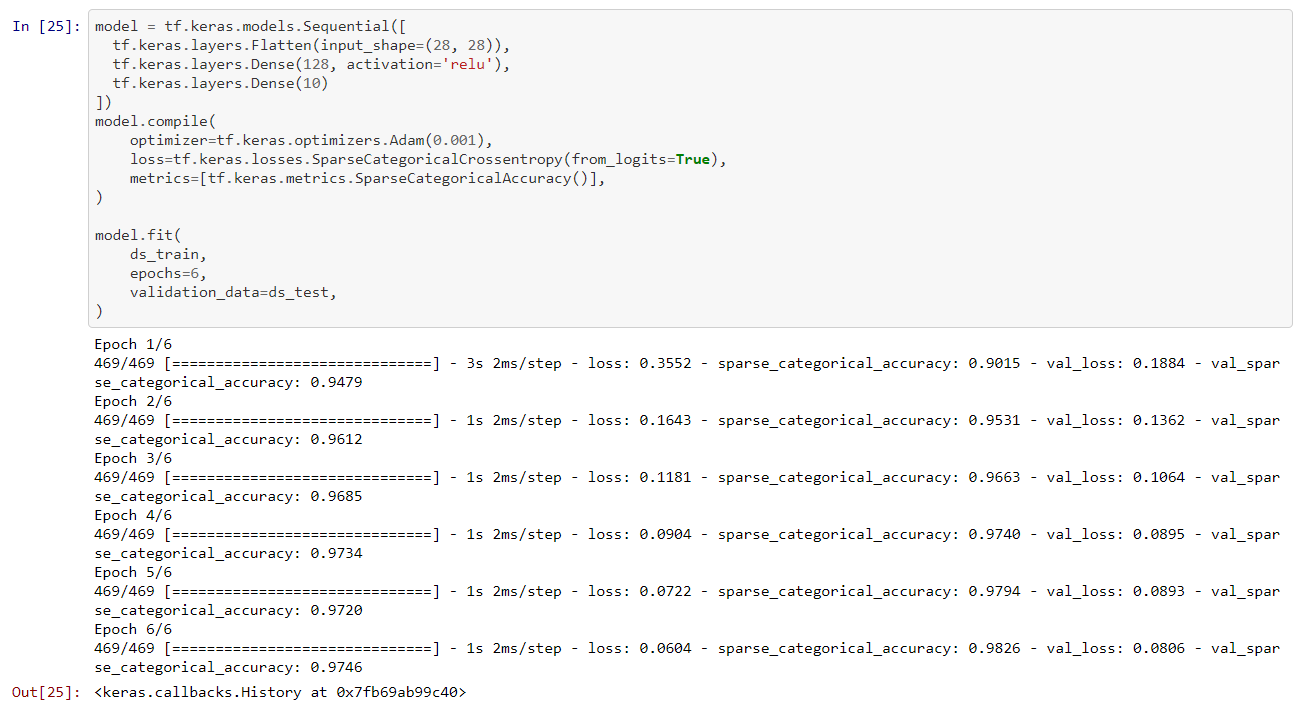
\includegraphics[width=0.95\textwidth]{t2.png} 
\caption{Tensorflow MNIST Training}
\label{Test}
\end{figure}

% \newpage
\newpage

\section{Convolutional Neural Networks}

在此將 CNN 歷年來重要的研究文獻整理如下所示 : 

\begin{center}
\begin{tabular}{ccccc}
\hline
方法名 & 年代 & 研究者 & 備註 \\
\hline
LeNet & 1998 & Y. Lecun et al. &  \\
AlexNet & 2012 & Alex Krizhevsky et al. &  \\
VGG & 2014.09 & Karen Simonyan et al. &  \\
Inception Net & 2014.09 & Christian Szegedy et al. & Google Inc. \\
Inception Net V2 & 2015.02 & Sergey Ioffe et al. & Google Inc. \\
Inception Net V3 & 2015.12 & Christian Szegedy et al. & Google Inc. \\
Inception Net V4 & 2016.02 & Christian Szegedy et al. & Google Inc. \\
Xception & 2016.10 & François Chollet & Google Inc. \\
ResNet & 2015.12 & Kaiming He et al. & Microsoft Research \\
DenseNet & 2016.08 & Gao Huang et al. &  \\
MobileNet V1 & 2017.04 & Andrew G. Howard et al. & Google Inc. \\
MobileNet V2 & 2018.01 & Mark Sandler et al. & Google Inc. \\
MobileNet V3 & 2019.05 & Andrew Howard et al. & Google AI, Google Brain \\
ShuffleNet V1 & 2017.07 & Xiangyu Zhang et al. & \\
ShuffleNet V2 & 2018.07 & Xiangyu Zhang et al.  & \\
\hline
\end{tabular}
\end{center}


\begin{enumerate}
\item Y. Lecun et al., Gradient-based learning applied to document recognition, LeNet, 1998.
\item Alex Krizhevsky et al., ImageNet Classification with Deep Convolutional Neural Networks, AlexNet, 2012.
\item Karen Simonyan et al., Very Deep Convolutional Networks for Large-Scale Image Recognition, VGG, 2014.
\item Christian Szegedy et al., Going Deeper with Convolutions, Inception Net, 2014, Google Inc.
\item Sergey Ioffe et al., Batch Normalization: Accelerating Deep Network Training by Reducing Internal Covariate Shift, Inception Net V2 , 2015, Google Inc.
\item Christian Szegedy et al., Rethinking the Inception Architecture for Computer Vision, Inception Net V3, 2015, Google Inc.
\item Christian Szegedy et al., Inception-v4, Inception-ResNet and the Impact of Residual Connections on Learning, Inception Net V4, 2016, Google Inc.
\item François Chollet, Xception: Deep Learning with Depthwise Separable Convolutions, Xception, 2016, Google Inc.
\item Kaiming He et al., Deep Residual Learning for Image Recognition, ResNet, 2015, Microsoft Research
\item Gao Huang et al., Densely Connected Convolutional Networks, DenseNet, 2016
\item Andrew G. Howard et al., MobileNets: Efficient Convolutional Neural Networks for Mobile Vision Applications, MobileNet V1, 2017, Google Inc.
\item Mark Sandler et al., MobileNetV2: Inverted Residuals and Linear Bottlenecks, MobileNet V2, 2018, Google Inc.
\item Andrew Howard et al., Searching for MobileNetV3, MobileNet V3, 2019, Google AI and Google Brain.
\item Xiangyu Zhang et al., ShuffleNet: An Extremely Efficient Convolutional Neural Network for Mobile Devices, ShuffleNet V1, 2017. 
\item Xiangyu Zhang et al., ShuffleNet V2: Practical Guidelines for Efficient CNN Architecture Design, ShuffleNet V2, 2018.
\end{enumerate}

% \newpage
\newpage

\section{附件 1}

下為 FC4-2 則在 Batch Size 為 30 時做到 0.961 的實際測試狀況。

\begin{verbatim}
Epoch:  0 | train loss: 2.3179 | test accuracy: 0.108
Epoch:  0 | train loss: 1.7215 | test accuracy: 0.438
Epoch:  0 | train loss: 0.9065 | test accuracy: 0.595
Epoch:  0 | train loss: 0.7863 | test accuracy: 0.695
Epoch:  0 | train loss: 0.7010 | test accuracy: 0.753
Epoch:  0 | train loss: 0.2025 | test accuracy: 0.772
Epoch:  0 | train loss: 0.5316 | test accuracy: 0.784
Epoch:  0 | train loss: 0.4025 | test accuracy: 0.808
Epoch:  0 | train loss: 0.4179 | test accuracy: 0.840
Epoch:  0 | train loss: 0.2629 | test accuracy: 0.851
Epoch:  0 | train loss: 0.5766 | test accuracy: 0.885
Epoch:  0 | train loss: 0.6210 | test accuracy: 0.878
Epoch:  0 | train loss: 0.3336 | test accuracy: 0.901
Epoch:  0 | train loss: 0.1728 | test accuracy: 0.917
Epoch:  0 | train loss: 0.2423 | test accuracy: 0.919
Epoch:  0 | train loss: 0.0907 | test accuracy: 0.932
Epoch:  0 | train loss: 0.1517 | test accuracy: 0.934
Epoch:  0 | train loss: 0.5776 | test accuracy: 0.928
Epoch:  0 | train loss: 0.2446 | test accuracy: 0.924
Epoch:  0 | train loss: 0.1774 | test accuracy: 0.938
Epoch:  0 | train loss: 0.1122 | test accuracy: 0.939
Epoch:  0 | train loss: 0.5981 | test accuracy: 0.932
Epoch:  0 | train loss: 0.0891 | test accuracy: 0.939
Epoch:  0 | train loss: 0.2379 | test accuracy: 0.941
Epoch:  0 | train loss: 0.1671 | test accuracy: 0.933
Epoch:  0 | train loss: 0.1797 | test accuracy: 0.945
Epoch:  0 | train loss: 0.2858 | test accuracy: 0.941
Epoch:  0 | train loss: 0.0684 | test accuracy: 0.942
Epoch:  0 | train loss: 0.1976 | test accuracy: 0.945
Epoch:  0 | train loss: 0.2697 | test accuracy: 0.941
Epoch:  0 | train loss: 0.1319 | test accuracy: 0.938
Epoch:  0 | train loss: 0.2735 | test accuracy: 0.947
Epoch:  0 | train loss: 0.2526 | test accuracy: 0.928
Epoch:  0 | train loss: 0.0490 | test accuracy: 0.934
Epoch:  1 | train loss: 0.0266 | test accuracy: 0.945
Epoch:  1 | train loss: 0.3994 | test accuracy: 0.949
Epoch:  1 | train loss: 0.4008 | test accuracy: 0.948
Epoch:  1 | train loss: 0.1298 | test accuracy: 0.954
Epoch:  1 | train loss: 0.1138 | test accuracy: 0.946
Epoch:  1 | train loss: 0.1101 | test accuracy: 0.953
Epoch:  1 | train loss: 0.0453 | test accuracy: 0.949
Epoch:  1 | train loss: 0.0528 | test accuracy: 0.955
Epoch:  1 | train loss: 0.0294 | test accuracy: 0.950
Epoch:  1 | train loss: 0.0197 | test accuracy: 0.949
Epoch:  1 | train loss: 0.1641 | test accuracy: 0.946
Epoch:  1 | train loss: 0.1442 | test accuracy: 0.937
Epoch:  1 | train loss: 0.2131 | test accuracy: 0.951
Epoch:  1 | train loss: 0.0344 | test accuracy: 0.950
Epoch:  1 | train loss: 0.1194 | test accuracy: 0.955
Epoch:  1 | train loss: 0.0861 | test accuracy: 0.952
Epoch:  1 | train loss: 0.6072 | test accuracy: 0.957
Epoch:  1 | train loss: 0.1805 | test accuracy: 0.952
Epoch:  1 | train loss: 0.0142 | test accuracy: 0.956
Epoch:  1 | train loss: 0.0102 | test accuracy: 0.953
Epoch:  1 | train loss: 0.3421 | test accuracy: 0.955
Epoch:  1 | train loss: 0.0862 | test accuracy: 0.952
Epoch:  1 | train loss: 0.3688 | test accuracy: 0.956
Epoch:  1 | train loss: 0.0111 | test accuracy: 0.954
Epoch:  1 | train loss: 0.3614 | test accuracy: 0.955
Epoch:  1 | train loss: 0.0869 | test accuracy: 0.952
Epoch:  1 | train loss: 0.0213 | test accuracy: 0.956
Epoch:  1 | train loss: 0.2109 | test accuracy: 0.962
Epoch:  1 | train loss: 0.2889 | test accuracy: 0.951
Epoch:  1 | train loss: 0.0637 | test accuracy: 0.962
Epoch:  1 | train loss: 0.0596 | test accuracy: 0.959
Epoch:  1 | train loss: 0.0034 | test accuracy: 0.965
Epoch:  1 | train loss: 0.0190 | test accuracy: 0.963
Epoch:  1 | train loss: 0.0153 | test accuracy: 0.961
tensor([7, 2, 1, 0, 4, 1, 4, 9, 6, 9]) prediction number
tensor([7, 2, 1, 0, 4, 1, 4, 9, 5, 9]) real number
\end{verbatim}

\newpage

\section{附件 2}

下為 FC4-1 在 Batch Size 為 50 時有 0.954 的實際測試狀況。

\begin{verbatim}
Epoch:  0 | train loss: 2.3079 | test accuracy: 0.105
Epoch:  0 | train loss: 1.2954 | test accuracy: 0.518
Epoch:  0 | train loss: 0.8506 | test accuracy: 0.718
Epoch:  0 | train loss: 0.4927 | test accuracy: 0.789
Epoch:  0 | train loss: 0.5421 | test accuracy: 0.832
Epoch:  0 | train loss: 0.3407 | test accuracy: 0.846
Epoch:  0 | train loss: 0.5657 | test accuracy: 0.848
Epoch:  0 | train loss: 0.3150 | test accuracy: 0.881
Epoch:  0 | train loss: 0.3149 | test accuracy: 0.882
Epoch:  0 | train loss: 0.7052 | test accuracy: 0.892
Epoch:  0 | train loss: 0.2937 | test accuracy: 0.905
Epoch:  0 | train loss: 0.3780 | test accuracy: 0.909
Epoch:  0 | train loss: 0.1319 | test accuracy: 0.919
Epoch:  0 | train loss: 0.2125 | test accuracy: 0.919
Epoch:  0 | train loss: 0.4903 | test accuracy: 0.915
Epoch:  0 | train loss: 0.0368 | test accuracy: 0.925
Epoch:  0 | train loss: 0.2886 | test accuracy: 0.925
Epoch:  0 | train loss: 0.3133 | test accuracy: 0.930
Epoch:  0 | train loss: 0.1374 | test accuracy: 0.927
Epoch:  0 | train loss: 0.2062 | test accuracy: 0.939
Epoch:  1 | train loss: 0.1921 | test accuracy: 0.937
Epoch:  1 | train loss: 0.2336 | test accuracy: 0.937
Epoch:  1 | train loss: 0.2420 | test accuracy: 0.937
Epoch:  1 | train loss: 0.0554 | test accuracy: 0.942
Epoch:  1 | train loss: 0.1244 | test accuracy: 0.938
Epoch:  1 | train loss: 0.0200 | test accuracy: 0.937
Epoch:  1 | train loss: 0.1651 | test accuracy: 0.947
Epoch:  1 | train loss: 0.1534 | test accuracy: 0.942
Epoch:  1 | train loss: 0.1084 | test accuracy: 0.947
Epoch:  1 | train loss: 0.1853 | test accuracy: 0.943
Epoch:  1 | train loss: 0.0954 | test accuracy: 0.951
Epoch:  1 | train loss: 0.2550 | test accuracy: 0.951
Epoch:  1 | train loss: 0.0765 | test accuracy: 0.946
Epoch:  1 | train loss: 0.3135 | test accuracy: 0.948
Epoch:  1 | train loss: 0.0769 | test accuracy: 0.948
Epoch:  1 | train loss: 0.2409 | test accuracy: 0.948
Epoch:  1 | train loss: 0.0431 | test accuracy: 0.952
Epoch:  1 | train loss: 0.0727 | test accuracy: 0.956
Epoch:  1 | train loss: 0.0572 | test accuracy: 0.948
Epoch:  1 | train loss: 0.1782 | test accuracy: 0.954
tensor([7, 2, 1, 0, 4, 1, 4, 9, 5, 9]) prediction number
tensor([7, 2, 1, 0, 4, 1, 4, 9, 5, 9]) real number
\end{verbatim}

\newpage

\section{附件 3}

Batch Size 為 50 ,EPOCH 為 10 ,加入卷積後改良的實際測試狀況。

\begin{verbatim}

Epoch:  0 | train loss: 2.3008 | test accuracy: 0.150
Epoch:  0 | train loss: 0.4211 | test accuracy: 0.836
Epoch:  0 | train loss: 0.1977 | test accuracy: 0.894
Epoch:  0 | train loss: 0.2739 | test accuracy: 0.895
Epoch:  0 | train loss: 0.2279 | test accuracy: 0.933
Epoch:  0 | train loss: 0.0972 | test accuracy: 0.938
Epoch:  0 | train loss: 0.2361 | test accuracy: 0.951
Epoch:  0 | train loss: 0.2102 | test accuracy: 0.957
Epoch:  0 | train loss: 0.0642 | test accuracy: 0.956
Epoch:  0 | train loss: 0.0603 | test accuracy: 0.951
Epoch:  0 | train loss: 0.1301 | test accuracy: 0.965
Epoch:  0 | train loss: 0.1806 | test accuracy: 0.959
Epoch:  0 | train loss: 0.1146 | test accuracy: 0.961
Epoch:  0 | train loss: 0.0452 | test accuracy: 0.965
Epoch:  0 | train loss: 0.0467 | test accuracy: 0.967
Epoch:  0 | train loss: 0.0450 | test accuracy: 0.971
Epoch:  0 | train loss: 0.1723 | test accuracy: 0.969
Epoch:  0 | train loss: 0.2110 | test accuracy: 0.969
Epoch:  0 | train loss: 0.1457 | test accuracy: 0.970
Epoch:  0 | train loss: 0.1125 | test accuracy: 0.973
Epoch:  1 | train loss: 0.1761 | test accuracy: 0.976
Epoch:  1 | train loss: 0.1053 | test accuracy: 0.971
Epoch:  1 | train loss: 0.0772 | test accuracy: 0.976
Epoch:  1 | train loss: 0.0253 | test accuracy: 0.975
Epoch:  1 | train loss: 0.0090 | test accuracy: 0.975
Epoch:  1 | train loss: 0.0401 | test accuracy: 0.976
Epoch:  1 | train loss: 0.0589 | test accuracy: 0.978
Epoch:  1 | train loss: 0.0169 | test accuracy: 0.976
Epoch:  1 | train loss: 0.0126 | test accuracy: 0.975
Epoch:  1 | train loss: 0.0848 | test accuracy: 0.977
Epoch:  1 | train loss: 0.0188 | test accuracy: 0.979
Epoch:  1 | train loss: 0.0560 | test accuracy: 0.980
Epoch:  1 | train loss: 0.0363 | test accuracy: 0.975
Epoch:  1 | train loss: 0.0170 | test accuracy: 0.982
Epoch:  1 | train loss: 0.0317 | test accuracy: 0.975
Epoch:  1 | train loss: 0.0755 | test accuracy: 0.983
Epoch:  1 | train loss: 0.0850 | test accuracy: 0.980
Epoch:  1 | train loss: 0.0484 | test accuracy: 0.982
Epoch:  1 | train loss: 0.0240 | test accuracy: 0.982
Epoch:  1 | train loss: 0.0183 | test accuracy: 0.982
Epoch:  2 | train loss: 0.0272 | test accuracy: 0.980
Epoch:  2 | train loss: 0.0021 | test accuracy: 0.983
Epoch:  2 | train loss: 0.0064 | test accuracy: 0.981
Epoch:  2 | train loss: 0.0182 | test accuracy: 0.984
Epoch:  2 | train loss: 0.0115 | test accuracy: 0.984
Epoch:  2 | train loss: 0.0075 | test accuracy: 0.979
Epoch:  2 | train loss: 0.0054 | test accuracy: 0.985
Epoch:  2 | train loss: 0.0064 | test accuracy: 0.982
Epoch:  2 | train loss: 0.0045 | test accuracy: 0.983
Epoch:  2 | train loss: 0.0987 | test accuracy: 0.981
Epoch:  2 | train loss: 0.0129 | test accuracy: 0.984
Epoch:  2 | train loss: 0.0289 | test accuracy: 0.983
Epoch:  2 | train loss: 0.0282 | test accuracy: 0.980
Epoch:  2 | train loss: 0.0262 | test accuracy: 0.984
Epoch:  2 | train loss: 0.0643 | test accuracy: 0.976
Epoch:  2 | train loss: 0.0618 | test accuracy: 0.984
Epoch:  2 | train loss: 0.0079 | test accuracy: 0.987
Epoch:  2 | train loss: 0.0912 | test accuracy: 0.984
Epoch:  2 | train loss: 0.0409 | test accuracy: 0.984
Epoch:  2 | train loss: 0.0788 | test accuracy: 0.982
Epoch:  3 | train loss: 0.0182 | test accuracy: 0.980
Epoch:  3 | train loss: 0.0124 | test accuracy: 0.984
Epoch:  3 | train loss: 0.0248 | test accuracy: 0.984
Epoch:  3 | train loss: 0.0077 | test accuracy: 0.984
Epoch:  3 | train loss: 0.0038 | test accuracy: 0.982
Epoch:  3 | train loss: 0.0444 | test accuracy: 0.988
Epoch:  3 | train loss: 0.1470 | test accuracy: 0.983
Epoch:  3 | train loss: 0.1792 | test accuracy: 0.985
Epoch:  3 | train loss: 0.0022 | test accuracy: 0.983
Epoch:  3 | train loss: 0.0345 | test accuracy: 0.986
Epoch:  3 | train loss: 0.0163 | test accuracy: 0.981
Epoch:  3 | train loss: 0.0084 | test accuracy: 0.984
Epoch:  3 | train loss: 0.0118 | test accuracy: 0.987
Epoch:  3 | train loss: 0.0162 | test accuracy: 0.985
Epoch:  3 | train loss: 0.0096 | test accuracy: 0.984
Epoch:  3 | train loss: 0.0072 | test accuracy: 0.980
Epoch:  3 | train loss: 0.0026 | test accuracy: 0.987
Epoch:  3 | train loss: 0.0025 | test accuracy: 0.987
Epoch:  3 | train loss: 0.1035 | test accuracy: 0.984
Epoch:  3 | train loss: 0.0082 | test accuracy: 0.984
Epoch:  4 | train loss: 0.0066 | test accuracy: 0.984
Epoch:  4 | train loss: 0.0099 | test accuracy: 0.987
Epoch:  4 | train loss: 0.0360 | test accuracy: 0.987
Epoch:  4 | train loss: 0.1021 | test accuracy: 0.981
Epoch:  4 | train loss: 0.0202 | test accuracy: 0.987
Epoch:  4 | train loss: 0.0013 | test accuracy: 0.984
Epoch:  4 | train loss: 0.0011 | test accuracy: 0.983
Epoch:  4 | train loss: 0.0125 | test accuracy: 0.986
Epoch:  4 | train loss: 0.0004 | test accuracy: 0.987
Epoch:  4 | train loss: 0.0045 | test accuracy: 0.983
Epoch:  4 | train loss: 0.0026 | test accuracy: 0.987
Epoch:  4 | train loss: 0.0232 | test accuracy: 0.981
Epoch:  4 | train loss: 0.0032 | test accuracy: 0.987
Epoch:  4 | train loss: 0.0013 | test accuracy: 0.988
Epoch:  4 | train loss: 0.0003 | test accuracy: 0.985
Epoch:  4 | train loss: 0.0051 | test accuracy: 0.984
Epoch:  4 | train loss: 0.0044 | test accuracy: 0.983
Epoch:  4 | train loss: 0.0118 | test accuracy: 0.985
Epoch:  4 | train loss: 0.0135 | test accuracy: 0.984
Epoch:  4 | train loss: 0.0563 | test accuracy: 0.984
Epoch:  5 | train loss: 0.0236 | test accuracy: 0.988
Epoch:  5 | train loss: 0.0005 | test accuracy: 0.987
Epoch:  5 | train loss: 0.0054 | test accuracy: 0.983
Epoch:  5 | train loss: 0.0042 | test accuracy: 0.989
Epoch:  5 | train loss: 0.0013 | test accuracy: 0.985
Epoch:  5 | train loss: 0.0023 | test accuracy: 0.985
Epoch:  5 | train loss: 0.0003 | test accuracy: 0.985
Epoch:  5 | train loss: 0.0038 | test accuracy: 0.982
Epoch:  5 | train loss: 0.0113 | test accuracy: 0.987
Epoch:  5 | train loss: 0.0019 | test accuracy: 0.985
Epoch:  5 | train loss: 0.0019 | test accuracy: 0.987
Epoch:  5 | train loss: 0.0026 | test accuracy: 0.985
Epoch:  5 | train loss: 0.0415 | test accuracy: 0.987
Epoch:  5 | train loss: 0.0559 | test accuracy: 0.986
Epoch:  5 | train loss: 0.0125 | test accuracy: 0.987
Epoch:  5 | train loss: 0.0121 | test accuracy: 0.984
Epoch:  5 | train loss: 0.0029 | test accuracy: 0.984
Epoch:  5 | train loss: 0.0102 | test accuracy: 0.984
Epoch:  5 | train loss: 0.0012 | test accuracy: 0.987
Epoch:  5 | train loss: 0.0365 | test accuracy: 0.983
Epoch:  6 | train loss: 0.0462 | test accuracy: 0.987
Epoch:  6 | train loss: 0.0074 | test accuracy: 0.984
Epoch:  6 | train loss: 0.0009 | test accuracy: 0.984
Epoch:  6 | train loss: 0.0004 | test accuracy: 0.984
Epoch:  6 | train loss: 0.0428 | test accuracy: 0.987
Epoch:  6 | train loss: 0.0032 | test accuracy: 0.989
Epoch:  6 | train loss: 0.0090 | test accuracy: 0.987
Epoch:  6 | train loss: 0.0009 | test accuracy: 0.985
Epoch:  6 | train loss: 0.0626 | test accuracy: 0.985
Epoch:  6 | train loss: 0.0674 | test accuracy: 0.987
Epoch:  6 | train loss: 0.0045 | test accuracy: 0.985
Epoch:  6 | train loss: 0.0087 | test accuracy: 0.988
Epoch:  6 | train loss: 0.0381 | test accuracy: 0.987
Epoch:  6 | train loss: 0.0868 | test accuracy: 0.985
Epoch:  6 | train loss: 0.0900 | test accuracy: 0.986
Epoch:  6 | train loss: 0.0019 | test accuracy: 0.984
Epoch:  6 | train loss: 0.0713 | test accuracy: 0.983
Epoch:  6 | train loss: 0.0020 | test accuracy: 0.984
Epoch:  6 | train loss: 0.0033 | test accuracy: 0.984
Epoch:  6 | train loss: 0.0039 | test accuracy: 0.986
Epoch:  7 | train loss: 0.0912 | test accuracy: 0.988
Epoch:  7 | train loss: 0.0018 | test accuracy: 0.985
Epoch:  7 | train loss: 0.0101 | test accuracy: 0.987
Epoch:  7 | train loss: 0.0012 | test accuracy: 0.985
Epoch:  7 | train loss: 0.0204 | test accuracy: 0.985
Epoch:  7 | train loss: 0.0012 | test accuracy: 0.987
Epoch:  7 | train loss: 0.0005 | test accuracy: 0.985
Epoch:  7 | train loss: 0.0208 | test accuracy: 0.985
Epoch:  7 | train loss: 0.0024 | test accuracy: 0.987
Epoch:  7 | train loss: 0.0509 | test accuracy: 0.987
Epoch:  7 | train loss: 0.0063 | test accuracy: 0.978
Epoch:  7 | train loss: 0.0007 | test accuracy: 0.988
Epoch:  7 | train loss: 0.0007 | test accuracy: 0.985
Epoch:  7 | train loss: 0.0056 | test accuracy: 0.986
Epoch:  7 | train loss: 0.0029 | test accuracy: 0.986
Epoch:  7 | train loss: 0.0469 | test accuracy: 0.988
Epoch:  7 | train loss: 0.0042 | test accuracy: 0.985
Epoch:  7 | train loss: 0.0139 | test accuracy: 0.986
Epoch:  7 | train loss: 0.0209 | test accuracy: 0.987
Epoch:  7 | train loss: 0.0569 | test accuracy: 0.986
Epoch:  8 | train loss: 0.0010 | test accuracy: 0.984
Epoch:  8 | train loss: 0.0007 | test accuracy: 0.988
Epoch:  8 | train loss: 0.0288 | test accuracy: 0.988
Epoch:  8 | train loss: 0.0009 | test accuracy: 0.985
Epoch:  8 | train loss: 0.0052 | test accuracy: 0.987
Epoch:  8 | train loss: 0.0008 | test accuracy: 0.988
Epoch:  8 | train loss: 0.0005 | test accuracy: 0.985
Epoch:  8 | train loss: 0.0049 | test accuracy: 0.987
Epoch:  8 | train loss: 0.0037 | test accuracy: 0.986
Epoch:  8 | train loss: 0.0060 | test accuracy: 0.984
Epoch:  8 | train loss: 0.0019 | test accuracy: 0.984
Epoch:  8 | train loss: 0.0017 | test accuracy: 0.986
Epoch:  8 | train loss: 0.0137 | test accuracy: 0.987
Epoch:  8 | train loss: 0.0018 | test accuracy: 0.988
Epoch:  8 | train loss: 0.0003 | test accuracy: 0.989
Epoch:  8 | train loss: 0.0186 | test accuracy: 0.985
Epoch:  8 | train loss: 0.0170 | test accuracy: 0.985
Epoch:  8 | train loss: 0.0005 | test accuracy: 0.980
Epoch:  8 | train loss: 0.0109 | test accuracy: 0.988
Epoch:  8 | train loss: 0.0004 | test accuracy: 0.989
Epoch:  9 | train loss: 0.0152 | test accuracy: 0.987
Epoch:  9 | train loss: 0.0130 | test accuracy: 0.987
Epoch:  9 | train loss: 0.0066 | test accuracy: 0.987
Epoch:  9 | train loss: 0.0027 | test accuracy: 0.988
Epoch:  9 | train loss: 0.0043 | test accuracy: 0.986
Epoch:  9 | train loss: 0.0088 | test accuracy: 0.987
Epoch:  9 | train loss: 0.0025 | test accuracy: 0.988
Epoch:  9 | train loss: 0.0029 | test accuracy: 0.988
Epoch:  9 | train loss: 0.0042 | test accuracy: 0.987
Epoch:  9 | train loss: 0.0001 | test accuracy: 0.987
Epoch:  9 | train loss: 0.0005 | test accuracy: 0.988
Epoch:  9 | train loss: 0.0038 | test accuracy: 0.985
Epoch:  9 | train loss: 0.0004 | test accuracy: 0.984
Epoch:  9 | train loss: 0.0063 | test accuracy: 0.985
Epoch:  9 | train loss: 0.0067 | test accuracy: 0.987
Epoch:  9 | train loss: 0.0169 | test accuracy: 0.984
Epoch:  9 | train loss: 0.0034 | test accuracy: 0.985
Epoch:  9 | train loss: 0.0027 | test accuracy: 0.985
Epoch:  9 | train loss: 0.0007 | test accuracy: 0.983
Epoch:  9 | train loss: 0.0641 | test accuracy: 0.984
tensor([7, 2, 1, 0, 4, 1, 4, 9, 5, 9]) prediction number
tensor([7, 2, 1, 0, 4, 1, 4, 9, 5, 9]) real number
\end{verbatim}

\clearpage

\end{document}